\documentclass[11pt]{article}
\usepackage{graphicx}
\usepackage[utf8]{inputenc}
\usepackage{fullpage}
\usepackage{hyperref}
\usepackage{natbib}
\usepackage{hyperref}
\usepackage{amsfonts}
\usepackage{graphicx}
\usepackage{hyperref}
\usepackage[utf8]{inputenc}
\usepackage{amsmath, amssymb, amsthm}
\usepackage{algorithm}
\usepackage{algpseudocode}
\usepackage{subcaption}
\usepackage{array}
\usepackage{listings}
\usepackage{xcolor}
\usepackage{geometry}

\theoremstyle{definition}
\newtheorem{definition}{Definition}

\title{Optimizing Healthcare Delivery: A Data-Driven Approach to Panel Size Management for Enhanced Patient Care at Vancouver Coastal Health}

\date{March 25th, 2024}


\begin{document}

\maketitle

\begin{abstract}

Vancouver Coastal Health (VCH) plays a significant role in delivering healthcare services across multiple community care centers in British Columbia. However, the optimal panel size for their Most Responsible Practitioners (MRP) poses a significant challenge, particularly in centers specializing in complex conditions. Currently, only five centers accommodate such patients, and the unique work schedules and part-time availability of MRPs complicate effective patient management.\\\\
This paper addresses the pressing concern of MRPs regarding workload and stress management, focusing on understanding the optimal panel size amidst diverse practitioner schedules. The project aims to explore the intricacies of panel size management, considering case complexity and practitioner availability. Achieving an optimal size is crucial for both MRP well-being and the overall improvement of healthcare services provided by VCH.\\\\
The primary objective of this project is to determine the optimal panel size for MRPs through detailed data analysis and simulation. By advocating for a smaller panel size, the project seeks to enhance the quality and efficiency of healthcare delivery. Additionally, it aims to provide insights into the impact of complexity scores on panel size and offer a data-driven justification for panel size variations compared to traditional family physicians.

\end{abstract}
\newpage
\section{Introduction}
Vancouver Coastal Health (VCH) stands at the forefront of healthcare delivery in British Columbia, encompassing a network of 19 community care centers. Among these, six primary care facilities specialize in addressing complex medical conditions, representing a cornerstone of the region's healthcare landscape. However, within this framework, a critical challenge emerges regarding the optimal panel size for their most responsible practitioners (MRPs). The current configuration sees only five centers equipped to handle patients with complex conditions, further complicated by the unique work schedules and part-time availability of MRPs.\\

This paper aims to address the pressing issue faced by VCH and its MRPs, focusing on the optimization of panel sizes to ensure efficient patient care delivery. The primary objective lies in delving into the complexities of panel size management, taking into account both the diverse schedules of practitioners and the intricacies of case complexity. By doing so, the paper seeks to provide a data-driven justification for optimal panel sizes, ultimately aiming to enhance the quality and efficiency of healthcare services provided by VCH. Through detailed data analysis and insights into the impact of case complexity on panel size, this study endeavors to offer practical solutions to the challenges faced by MRPs and contribute to the ongoing improvement of healthcare delivery within the VCH network.\\

\section{Literature Review}

The optimal panel size for primary care practitioners is a critical factor in ensuring high-quality healthcare delivery and practitioner well-being. Not only does it impact client outcomes, but it also directly influences the workload and stress levels experienced by healthcare providers. Previous studies have highlighted the importance of balancing patient load with the capacity of healthcare providers to deliver effective and timely care \cite{dahrouge2016, harrington2022}. This balance is essential for maintaining the quality of care while safeguarding the physical and mental well-being of healthcare professionals. As such, understanding the factors that contribute to determining the optimal panel size is of paramount importance in healthcare management. In this literature review, we delve into existing research to explore the complexities surrounding panel size optimization and its implications for healthcare delivery, with a particular focus on the context of Vancouver Coastal Health (VCH). Through this examination, we aim to provide valuable insights that can inform strategies for enhancing patient-centered care and promoting the satisfaction and effectiveness of healthcare providers within VCH and similar healthcare organizations.\\

\cite{dahrouge2016} emphasized that a well-managed panel size is associated with improved quality of care, underscoring the need for a data-driven approach to determining panel sizes that can sustain high-quality patient outcomes.\\

The complexity and vulnerability of patient populations, particularly in urban areas like the Vancouver Coastal Health region, necessitate a nuanced understanding of panel size management \cite{shukor2018}. These populations often require more intensive and coordinated care efforts, which can strain the resources and capacities of healthcare providers. \cite{shukor2018} discuss the development of community-based primary healthcare initiatives aimed at addressing these challenges, indicating the relevance of innovative care models in complex healthcare environments.\\

Furthermore, capacity management extends beyond primary care into broader organizational contexts. Elkhuizen et al. \cite{elkhuizen2007} explored capacity management of nursing staff as a means for organizational improvement, suggesting that optimal staffing levels can enhance operational efficiency and patient care quality. This principle can be applied to the management of MRPs’ panel sizes, where effective capacity planning is essential for maintaining service quality and practitioner satisfaction.\\

Research on the operationalization of high-performing primary care through analytics tools \cite{joe2020} demonstrates the potential of data-driven strategies to enhance healthcare delivery. By leveraging detailed analytics, healthcare organizations can identify optimal panel sizes that balance practitioner workload with patient care needs, fostering a sustainable healthcare delivery model.\\\\
Moreover, the optimization of nurse schedules at community health centers represents another facet of capacity management within healthcare settings. \cite{zimmerman2021} presented a novel scheduling approach to align nurse shifts with client demand at an inner-city community health center, improving access to care without increasing total nurse staffing levels. This innovative approach highlights the importance of strategic scheduling in addressing operational concerns and improving patient outcomes.\\\\
Systematic reviews and studies on hospital capacity planning and optimization further support the need for strategic panel size management \cite{shekelle2019, humphreys2022, zhu2019}. These works highlight the dynamic nature of healthcare delivery systems and the importance of adaptable strategies to manage practitioner workload and patient care quality effectively.\\\\
In addition to emphasizing the criticality of optimal panel size for primary care practitioners, it's essential to acknowledge the rising importance of multimorbidity in healthcare. Multimorbidity, the presence of two or more chronic conditions within an individual, poses diverse challenges to patients, including functional decline, mental health issues, polypharmacy, and heightened risk of severe COVID-19. High-quality primary care plays a crucial role in effectively addressing the complex healthcare needs associated with multimorbidity in a cost-effective manner. Primary care is particularly vital for improving population health outcomes and ensuring continuity of care for individuals with multiple chronic conditions. Therefore, understanding and optimizing panel sizes for primary care practitioners are paramount, as they directly impact the capacity to deliver comprehensive care to patients with multimorbidity. Incorporating insights from multimorbidity studies into panel size optimization strategies allows healthcare organizations to align resources and capacities to meet evolving patient needs while safeguarding the well-being of healthcare providers.\cite{hu2022}\\\\
\cite{Harrington2021} delves into panel size management in healthcare systems, focusing on workload balancing among providers. It considers key factors such as the ratio of a primary care provider's workload to their daily capacity, patient characteristics, and practical constraints on patient transfers. A strategic approach is proposed, involving patient panel reassignment and, if needed, the hiring of new providers to achieve workload balance without exceeding a predefined threshold for provider utilization. Drawing on data from a Louisville regional healthcare system, an integer linear program model is developed to address this issue. Three case studies based on this data highlight the effectiveness of the proposed model in achieving load balancing and preventing physician burnout \cite{Harrington2021}.This strategic approach offers valuable insights into optimizing healthcare delivery by efficiently managing provider workloads while ensuring quality patient care.\\

\cite{edwards2018} conducted a cross-sectional study focusing on small-to-medium-sized primary care practices across seven regions of the United States. The study aimed to evaluate burnout among healthcare providers within these practices. They found that provider experience and burnout were significant factors in these settings, highlighting the potential impact of panel size and workload on healthcare professionals' well-being and job satisfaction. The clustering of practices allowed for a nuanced understanding of how organizational factors contribute to burnout, shedding light on the importance of effective panel size management in optimizing the work environment for healthcare providers.\\\\
\cite{francis2009effect} conducted a cross-sectional study involving 40 internal medicine residents, with patient data not reported. The study aimed to assess patient continuity within internal medicine residency programs. They found that the number of clinics attended by a resident had an impact on patient continuity, indicating a potential association between panel size and the ability of residents to maintain continuity of care for their patients. This suggests that optimizing panel size within residency programs may contribute to better patient care experiences and outcome.\\\\
\cite{Helfrich2017} conducted a cross-sectional study involving primary care providers, nurse care managers, clinical associates, and administrative clerks from a national VA sample, revealing that 31.6 of panels exceeded the capacity of over 1,200 patients. Provider burnout was positively associated with workload indicators such as team staffing ratios and working on multiple teams. \cite{kamnetz2018} conducted an observational study involving 112 primary care physicians in 27 clinics, showing that active patient panel weighting increased access, ensuring appointments were available when needed in family or general internal medicine.\\\\
Panel size management in primary care is a critical aspect of healthcare delivery, influencing both patient outcomes and provider satisfaction. Several studies have investigated the impact of panel size on various aspects of care provision. For instance, \cite{Angstman2016} examined the relationship between family medicine panel size and care quality, highlighting the importance of appropriately sized panels for maintaining high-quality care. \cite{Rajkomar2016} proposed a novel electronic health record-derived measure using machine learning to weight primary care patient panel sizes, emphasizing the need for accurate and efficient methods to manage panel sizes. Additionally, \cite{Hirozawa2016} conducted multivariate risk adjustment of primary care patient panels, underscoring the complexity of panel size management in public health settings. These articles collectively contribute to our understanding of the challenges and strategies involved in optimizing panel sizes to enhance patient-centered care and mitigate provider burnout.\\\\
The reviewed studies utilize various methodologies to investigate panel size optimization in healthcare, including mathematical modeling, simulation techniques, and empirical analyses. While mathematical modeling, as seen in studies by \cite{dahrouge2016} and \cite{joe2020}, offers systematic exploration of optimal panel sizes, it may oversimplify real-world complexities and rely heavily on assumptions. Simulation techniques, demonstrated by \cite{shukor2018} and \cite{zimmerman2021}, provide flexibility for testing different approaches but require accurate input data and assumptions. Empirical analyses, like those by \cite{elkhuizen2007}, offer direct evidence but may be constrained by data availability and quality. Despite these findings, gaps and limitations persist in the literature. Large-scale, longitudinal studies are scarce, hindering generalizable conclusions on panel size optimization's impact. Additionally, methodological biases and the lack of standardized measurement make comparison challenging. Overlooking factors such as patient demographics and organizational culture further complicates the issue. Our research, inspired by previous studies, focuses on the optimal panel size for primary care practitioners within Vancouver Coastal Health (VCH). By incorporating advanced analytics and stakeholder perspectives, we aim to provide empirical evidence and develop evidence-based strategies for improving healthcare delivery within VCH and similar organizations.\\\\
In conclusion, the literature underscores the complexity of determining the optimal panel size for healthcare providers, considering factors such as patient complexity, practitioner well-being, and organizational efficiency. This review sets the stage for our study’s contribution to the field, aiming to provide a data-driven analysis of panel size optimization within the Vancouver Coastal Health network, addressing both the challenges of case complexity and the critical need for maintaining high-quality patient care and practitioner well-being.

\section{Background}

Vancouver Coastal Health (VCH) employs a Panel Size Planning (PSP) approach to calculate the ideal panel sizes for Most Responsible Practitioners (MRPs). This method hinges on average metrics, such as the average number of patient visits per year, to estimate the workload manageable by healthcare providers. At its core, the PSP formula aims to balance the demand for patient visits against the provider's capacity to deliver care, encapsulated in the formula: Ideal Panel Size = (Provider visits per day * Provider days per year) / Average visits per patient per year. \cite{PanelManagement2018} \\\\
This calculation method, while straightforward, has notable limitations. Primarily, it relies excessively on general averages, failing to account for the diverse care needs and complexity of individual patients. Given the varied and often complex health conditions of the patient population served by VCH, particularly those with multimorbidity, a one-size-fits-all approach to panel size calculation falls short. The current PSP method does not differentiate between patients requiring simple annual check-ups and those needing frequent, specialized care, nor does it adjust for the part-time availability and unique work schedules of MRPs.\\\\
Moreover, the PSP approach overlooks critical contextual factors, such as the demographic characteristics of the patient population and the socioeconomic status of the community served. These factors can significantly impact healthcare needs and service demand, making a rigid formulaic approach to panel size planning inadequate. The method's reliance on historical data for panel size adjustments also renders it fundamentally reactive, limiting its capacity to anticipate and adapt to future changes in healthcare demand or provider availability.\\\\
Another critical limitation is the PSP's simplification of healthcare dynamics into basic averages. This oversimplification potentially neglects the intricate interactions and dependencies within healthcare systems, affecting client care and provider workload. Additionally, the approach offers limited customization options, restricting the ability to tailor panel sizes based on specific patient population characteristics, and may result in longer wait times for appointments due to an imbalanced allocation of patient load.\\\\
Given these limitations, there is a pressing need for a more sophisticated, adaptable method for calculating panel sizes at VCH. The implementation of a discrete event simulation model, leveraging detailed data analysis and accommodating the complex interplay of patient demand and provider capacity, could offer a more nuanced, efficient, and responsive approach to panel size planning. This model would not only address the limitations of the PSP approach but also enhance the quality and efficiency of healthcare delivery, ensuring that MRPs can manage their workloads effectively while meeting the diverse healthcare needs of their patients.   

\subsection*{Our Approach}
The PSP approach, fundamentally rooted in averages, falls short in differentiating the distinct requirements of individual patients, especially considering the diverse demographic and socioeconomic contexts within which they reside. Its reliance on historical data also meant that the system's ability to preemptively adjust to shifting demands and provider availabilities was limited, essentially making it a reactive model rather than a proactive one.\\\\
In light of these limitations, our revised approach is anchored in Discrete Event Simulation (DES). This sophisticated modeling technique allows us to simulate the operation of healthcare systems as a sequence of discrete, individual events, each occurring at distinct time points and altering the state of the system. DES encompasses the unpredictability of patient arrivals and service demands, thus offering a predictive, adaptive, and realistic modeling of patient flow and MRP service demand. \cite{Robinson2020}\\\\ To this end, we implement a Poisson Process Queueing System (PPQS) to better accommodate the randomness in patient arrivals and the variability in appointment duration. This model is equipped to handle the inherent non-uniformity of healthcare delivery, incorporating the full spectrum of complexity scores and the probabilistic nature of no-shows. By integrating these factors, our approach is designed to provide a granular analysis of service utilization rates, waiting times, and patient loads—ensuring that MRPs are better positioned to manage their workload effectively while delivering high-quality care tailored to each patient's unique needs.\\\\
Moreover, the flexibility of the DES model allows for quick adjustments and customization based on real-time data analysis, offering a versatile tool in the face of evolving healthcare demands. By incorporating a systematic consideration for randomness and patient behavior patterns, such as no-shows, the model becomes highly responsive to the dynamic nature of clinical settings.\\\\
Our revised approach, therefore, shifts from the static, average-based calculations of the PSP to a dynamic DES framework. This model not only captures the intricate dynamics of healthcare systems but also enhances the capacity for immediate, data-driven responses to changes in patient behavior and care requirements. It is a significant step towards a more resilient and patient-centric healthcare system, aligning MRP workloads with the actualized patterns of patient demand. \cite{Ansell2017}\\\\
As we implement this DES-based panel size planning, we anticipate a reduction in wait times and an improvement in the allocation of resources. This aligns with our commitment to optimizing operational efficiency while maintaining the standard of care that VCH is known for. Our approach underscores the potential of advanced simulation models in transforming healthcare operations, paving the way for a future where healthcare systems are as dynamic and complex as the patients they serve.\\\\
\section{Problem Statement}

Our goal is to determine the optimal panel size for Vancouver Coastal Health (VCH), but we have two primary concerns:

\begin{enumerate}
    \item \textbf{Quality of Service for Patients:} It is crucial to ensure that the quality of service provided to patients remains high. This entails balancing patient load with the capacity of MRPs to deliver effective and timely care. Failure to maintain high-quality service risks compromising patient outcomes and satisfaction.
    
    \item \textbf{Practitioner Well-being:} MRPs may experience fatigue and overwork if they are required to see too many patients within limited working hours. Managing workload effectively is essential to prevent burnout and maintain the well-being and effectiveness of MRPs within the VCH healthcare network.
\end{enumerate}

These concerns highlight the importance of optimizing panel sizes while considering both patient care quality and practitioner well-being. Failure to address these issues could lead to negative consequences for both patients and MRPs. Thus, our objective is to determine an optimal panel size that addresses these concerns and ensures the continued delivery of high-quality healthcare services at VCH.\\\\
In the Vancouver Coastal Health (VCH) network, primary care clinics are grappling with the critical challenge of determining the optimal panel size for Most Responsible Practitioners (MRPs) amid a landscape marked by an increasing complexity of patient needs and a scarcity of healthcare providers. The current static and average-based panel size calculation method, aiming for a target of 1200 patients per MRP, does not account for the dynamic nature of healthcare demand, the wide range of patient complexities, nor the limited and variable availability of MRPs, many of whom do not work full-time. This discrepancy between the theoretical panel size and the practical limitations has led to a significantly lower  actual panel sizes, with MRPs managing as few as 200 patients, thereby having access issues for primary care, particularly for vulnerable populations with complex healthcare needs, including those unhoused or living in shelters.\\\\
The inadequacy of the current panel size model to reflect the real-world variability and complexity of patient care needs hampers efficient resource allocation, affects the quality of care, and limits access to healthcare services. Furthermore, the existing approach lacks a mechanism to incorporate critical contextual factors such as patient demographics, healthcare utilization patterns, and the interdisciplinary nature of modern primary care, which includes team-based approaches and the integration of social determinants of health into patient care planning.\\\\
Therefore, there is an urgent need for a sophisticated, data-driven model that can dynamically adjust to the complexities of patient needs and healthcare provider capacities. Such a model would not only facilitate more accurate and flexible panel size planning but also support VCH’s strategic objectives of enhancing access to primary care, improving healthcare delivery efficiency, and ensuring equitable healthcare services for all community members, especially the most vulnerable.


\section{Data Analysis}

To achieve the primary objective of determining the optimal panel size for Most Responsible Practitioners (MRPs) within Vancouver Coastal Health (VCH) and to evaluate the impact of case complexity on healthcare delivery, we employed a comprehensive data analysis strategy. This strategy was informed by analyzing the Electronic Medical Records (EMR) data provided by Vancouver Coastal Health (VCH).\\\\
Our data analysis commences with the determination of two pivotal metrics: lambda ($\lambda$) and the Complexity Score Index (CSI), which are instrumental for understanding the demand on healthcare services and the complexity of care required for appointments that are actively kept by patients.\\\\
\textbf{Booking Rate Calculation ($\lambda$):}\\\\
Lambda ($\lambda$) is a measure that reflects the average number of appointment requests per patient per month. To calculate lambda, we begin by importing appointment data into a dataframe from an Excel file containing patient identifiers, appointment dates, and descriptions of appointment types. Each record in this dataset corresponds to a patient's appointment, providing us with a foundational basis for our analysis.\\\\
From this dataset, we filter out appointment types that are classified as walk-ins or administrative kind to focus on the booked or scheduled appointments. This exclusion is crucial to ensure that lambda accurately represents the frequency of healthcare utilization rather than inflated numbers due to non-attendance or administrative bookings.\\\\
With the filtered data, we proceed to calculate lambda. This is done by grouping the data by patient identifier (PID) and counting the number of appointments per patient. We then divide this count by the total number of months covered in the data set, which spans from April 2021 to January 2024. The result is a lambda value for each patient that serves as a quantifiable metric of their monthly demand on the healthcare system.\\\\
\textbf{Complexity Score Index (CSI):}\\\\
Concurrently, we assess the complexity of each patient's healthcare needs through the CSI. The CSI data, extracted from a separate dataset, consists of a score for each patient which is reflective of their health condition's complexity. To derive a singular, aggregate complexity score for each patient, we compute the average of their CSI scores.\\\\
The average CSI for each patient is then linked with their corresponding lambda value. This linkage forms the basis for analyzing the relationship between the rate at which patients book appointments and the complexity of their healthcare needs.\\\\
Both lambda and CSI values are critical in informing our understanding of healthcare demand and patient complexity.\\\\
\textbf{They provide a dual perspective on patient behavior:}
\begin{enumerate}
    \item One that informs on the frequency of healthcare engagement.
    \item And another on the complexity of care that patients require.
\end{enumerate}
By analyzing these measures for booked appointments only, we gain insights into actual healthcare service utilization, stripping away potential data distortions from unattended or non-clinical interactions.This comprehensive view is essential for optimizing panel sizes and enhancing the delivery of care within the healthcare system.

\begin{figure}[H]
    \centering
    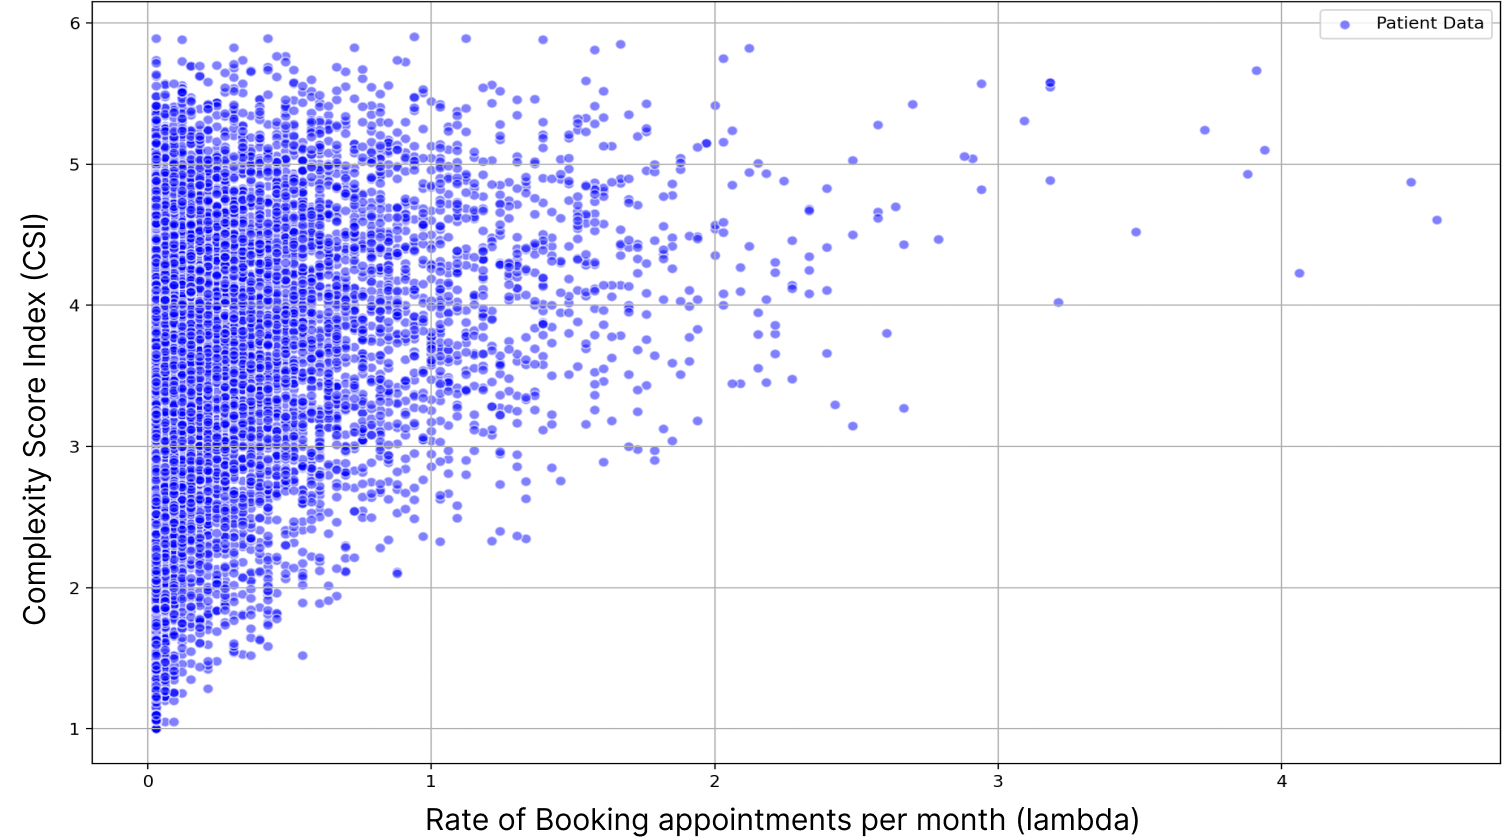
\includegraphics[width=1\textwidth]{CSI vs Lambda.png}
    \caption{Relationship between Lambda (Booking Rate) and CSI (Complexity Score Index) for Booked Appointments Only.}
    \label{fig:lambda_csi}
\end{figure}

The accompanying scatter plot illustrates the relationship between lambda (the rate of booking appointments per month) and the Complexity Score Index (CSI), presenting a discernible trend. Predominantly, the data points are concentrated at lower lambda values, indicating that the majority of patients book fewer than one appointment per month, regardless of the complexity of their healthcare needs. This concentration at lower lambda values could suggest that patients with more complex needs may opt for walk-in appointments as opposed to scheduled bookings, a trend that could reflect the urgent or unpredictable nature of their healthcare requirements.\\\\
It is noteworthy that as lambda values increase—indicating more frequent bookings—there is a visible spread in the CSI values. This spread could imply that patients with higher healthcare needs, who are booking appointments more frequently, exhibit a broad spectrum of complexity in their conditions. This variance in complexity at higher levels of healthcare engagement underscores the multifaceted challenges MRPs face when scheduling and providing care. It also hints at the necessity for a flexible and responsive appointment system that can accommodate the unpredictable patterns of high-need patients.\\\\
\textbf{Show Rate for Patients: }
The 'ShowRate' metric is a critical indicator of patient adherence to scheduled healthcare appointments. This 'Show rate' is calculated by analyzing appointment data for each patient, focusing on the critical question: when an appointment is scheduled, how often does the patient show up?\\\\
The 'ShowRate' metric emerges as a pivotal gauge of patient engagement and adherence, as underscored in a study published in the Health Informatics Journal \citep{lacy2011appointment}. The significance of 'ShowRate' is rooted in its capacity to mirror the actual utilization of scheduled healthcare services. It is a direct measure of the frequency at which patients follow through on their appointments, a behavioral pattern that holds substantial implications for resource optimization within healthcare systems.\\\\
The aforementioned study by Lacy and colleagues delves into the ramifications of no-shows for outpatient appointments, elucidating the ensuing operational inefficiencies and financial strains. As such, the 'ShowRate' provides healthcare facilities with invaluable insights, enabling them to calibrate their scheduling systems, predict potential gaps in service utilization, and devise strategies to mitigate the impact of missed appointments.\\\\
To compute the 'ShowRate', we initially gather the data from EMR data provided to us, which provides us with individual records, each marking a patient's decision to either attend ('show') or miss ('no-show') their appointment. The data includes patient identifiers, the occurrence of the appointment, and a descriptor of the appointment's nature.\\\\
Acknowledging the importance of analyzing genuine attempts at seeking healthcare, we exclude appointment types from our dataset that are classified as walk-ins or administrative kind. This exclusion criterion is essential to distill the true essence of 'ShowRate' for booked appointments. The excluded types encompass various non-clinical interactions such as phone calls, walk-ins for non-medical reasons, administrative notes, and other such activities.\\\\
With the refined dataset, we proceed to calculate the 'ShowRate' by grouping the data by patient identifier (PID) and determining the mean of the \text{"is\_visit"} variable. The \text{"is\_visit"} variable is binary, with '1' indicating a patient's attendance to an appointment and '0' for absence. By calculating the average of this binary variable, we essentially measure the proportion of times a patient is present for their appointments out of the total number of appointments scheduled for them. The resultant 'ShowRate' ranges from 0 to 1, where '1' signifies perfect attendance and values closer to '0' indicate higher frequencies of no-shows.\\\\
The computation yields a 'ShowRate' for each patient, serving as a quantitative reflection of their reliability in attending scheduled appointments. This rate is not only indicative of patient behavior but also plays a significant role in understanding and managing healthcare resources effectively, as it directly impacts scheduling dynamics and resource allocation.

\begin{figure}[H]
    \centering
    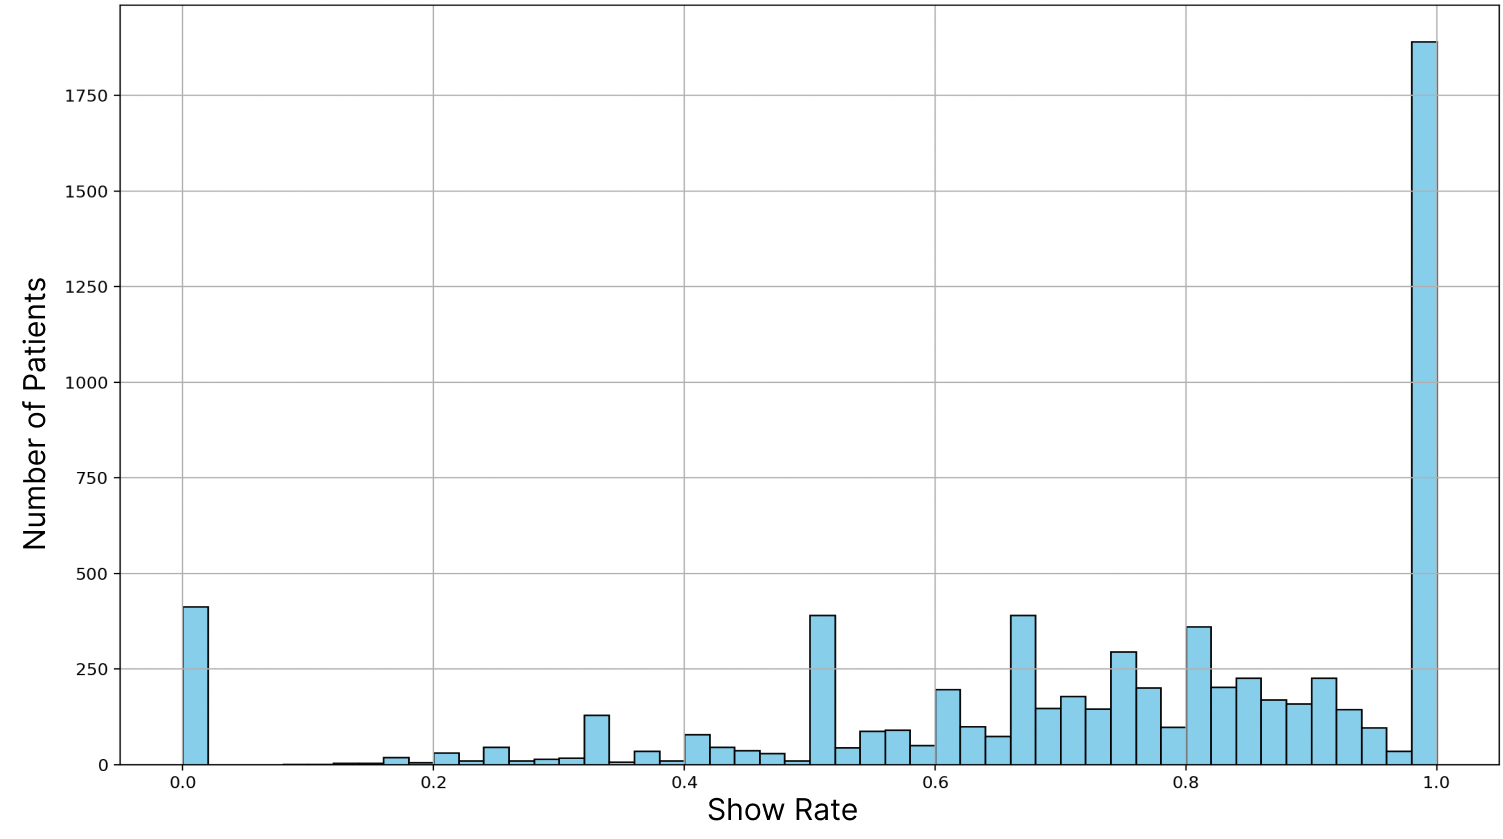
\includegraphics[width=1\textwidth]{noShow Distribution.png}
    \caption{Distribution of Patient Show Rates.}
    \label{fig:show_rate}
\end{figure}

As evidenced by the histogram of patient show rates, there is a substantial concentration of patients with show rates near 1, indicating a majority who consistently attend their appointments. However, the distribution also reveals a segment of the patient population with show rates less than 1, emphasizing the challenge of no-shows in resource allocation and scheduling for MRPs.\\\\
Our methodological backbone resides in the pragmatic scheduling ethos of MRPs. Despite initial assessments of weekly work hours, our simulation framework pivots on the concrete availability for patient appointments—predicated on first-hand insights from practitioners, affirming a six-hour daily window earmarked for consultations, each typically spanning thirty minutes. This finding corroborates our fixed-time simulation paradigm.\\\\
Synthesizing these elements, our simulations stride towards ascertaining an ideal panel size, one that upholds the caliber of patient care alongside MRP welfare. Addressing the substantial role of no-shows—revealed by our data as a significant operational factor—our simulations aspire to harmonize patient needs with MRP capacity.\\\\
In sum, the amalgamation of calculated lambda values, CSI scores, and 'ShowRate' creates a robust dataset from which we can explore the many facets of healthcare demand and supply. By understanding these dynamics, we can move toward an optimally balanced healthcare system that meets the needs of all parties involved.

\section{Model}

\subsection*{Simulation for Determining Optimal Panel Size}

In addressing the critical issue of determining the optimal panel size for Most Responsible Practitioners (MRPs) at Vancouver Coastal Health (VCH), we have constructed a comprehensive simulation model. This model, which utilizes discrete-event simulation (DES), a stochastic modeling approach widely used to address dynamic and complex systems such as healthcare \cite{Vázquez-Serrano2021}, is instrumental in evaluating how fluctuations in panel size directly impact the mean waiting time for appointments. Our objective is to maintain a delicate equilibrium between ensuring high-quality patient care and preserving the welfare of healthcare practitioners. By conducting rigorous simulations of various panel sizes under a range of conditions, our methodology is predicated on delivering a meticulously devised, data-driven solution to enhance healthcare delivery within the VCH network.

\subsection*{Methodology}
At the core of our simulation is the complex computation of the mean patient wait time across a variety of panel sizes. In this context, the panel size refers to the number of patients under the care of a single Most Responsible Practitioner (MRP), a key determinant in the efficacy of healthcare delivery. Our model makes use of a discrete event simulation technique, which is highly regarded for its ability to represent the dynamic character of systems in which events occur at discrete times. We precisely simulate patient appointment requests, which are a crucial part of healthcare scheduling, by using the Poisson distribution \cite{Leeftink2021}. The simulation's settings are deliberately selected to cover essential aspects of healthcare operations, such as the MRP's weekly availability and the total number of appointment slots available throughout the simulated time. \\\\
By implementing a discrete event simulation approach, our model precisely captures the complex interaction between patient demand and MRP availability, providing invaluable insights into the operational dynamics of healthcare delivery. Through the application of the Poisson distribution, we effectively model the stochastic nature of appointment requests, recognizing the inherent variability in patient arrival patterns. This allows us to simulate realistic scenarios that closely reflect the complexities of real-world healthcare environments. \\\\
To further guarantee that our model is firmly rooted in the reality of healthcare operations, we carefully select our simulation parameters to capture crucial features of healthcare scheduling and resource allocation. We interviewed healthcare workers actively involved in patient care within the Vancouver Coastal Health (VCH) network to get insightful information about the real-world challenges they confront. Notably, we had the honor of speaking with renowned VCH MRP Dr. Steven Yau, who offers priceless insights on the difficulties involved with managing patient panels. \\\\
It was revealed to us during our discussion with Dr. Yau that he sees patients two days a week, working part-time. There are two separate sessions every day; Dr. Yau sees patients for three hours in the morning and three more hours in the afternoon. Thanks to our thorough comprehension of Dr. Yau's work schedule, we were able to precisely replicate the subtleties of healthcare scheduling in our simulation model.\\\\
We incorporated Dr. Yau's part-time schedule, which is important information, into our simulation settings. Our simulation guarantees a realistic portrayal of the operational restrictions experienced by healthcare practitioners by faithfully simulating the MRP's weekly availability, which corresponds to Dr. Yau's work schedule. This addition strengthens the validity and applicability of our findings by demonstrating our dedication to creating a simulation model that closely mimics the complexities of actual healthcare settings.
\begin{itemize}
    \item \textbf{Poisson Distribution:} The Poisson distribution serves as a fundamental mathematical concept utilized in our simulation model to accurately model the number of appointment requests from patients. This probability distribution is particularly well-suited for scenarios where events occur randomly and independently over a continuous interval of time, making it an ideal choice for simulating the stochastic nature of patient appointment requests within healthcare settings. \\\\
    In our simulation, each patient is assigned a lambda ($\lambda$) value, which represents the average number of appointment requests they generate per week. This lambda value encapsulates various factors such as the patient's medical needs, frequency of follow-up visits, and overall healthcare utilization patterns. By assigning lambda values to individual patients and aggregating these values across the entire patient panel, we effectively simulate the total appointment demand placed on MRPs within the VCH network.
    
    The aggregation of lambda values allows us to capture the collective appointment request behavior of all patients under the care of a single MRP. This comprehensive approach enables us to accurately model the dynamic nature of patient demand and assess its impact on healthcare capacity and scheduling efficiency. By simulating the total appointment demand across the panel, we gain valuable insights into the workload faced by MRPs and can make informed decisions regarding panel size optimization to ensure timely and effective patient care delivery. \\\\
    In essence, the Poisson distribution, coupled with lambda values assigned to individual patients, forms the cornerstone of our simulation methodology. By leveraging this mathematical framework, we are able to simulate realistic scenarios that closely mirror the complexities of patient appointment scheduling within the healthcare environment. This allows us to provide actionable insights into panel size optimization strategies aimed at enhancing healthcare delivery efficiency and improving patient outcomes within the VCH network.

    \item \textbf{Simulation Parameters:} In our simulation model, several key parameters are carefully defined to accurately reflect the operational dynamics of healthcare delivery within the Vancouver Coastal Health (VCH) network. These parameters play a crucial role in shaping the simulation environment and ensuring that our model remains aligned with the realities of healthcare scheduling and resource allocation.
    
    \begin{itemize}
    \item \textbf{MRP Availability:} First and foremost, we consider the availability of Most Responsible Practitioners (MRPs), which is defined as 12 hours per week. This availability is distributed across two days, with each day comprising six hours of MRP availability. This allocation of MRP availability reflects the practical constraints faced by healthcare practitioners, acknowledging the need to balance patient care responsibilities with other professional commitments. By accurately defining MRP availability, we ensure that our simulation captures the realistic workload distribution faced by MRPs within the VCH network.
    \item \textbf{Appointment Slots:} Additionally, we define the number of appointment slots available within the simulation period. Each appointment is assumed to last 30 minutes, resulting in a total of 24 appointment slots available per week. This allocation of appointment slots reflects the typical duration of patient appointments within primary care settings and allows us to effectively manage patient flow within the simulated environment. By considering the finite availability of appointment slots, we can accurately assess the impact of panel size variations on patient wait times and healthcare capacity.
    \item \textbf {Simulation Period:} Furthermore, the simulation period is now defined to encompass a sixteen-week period. This extended duration allows us to capture a larger volume of appointment requests and assess the long-term implications of panel size optimization strategies more effectively. By simulating appointment requests over this multi-week period, we can identify more robust trends and patterns in patient demand. This facilitates more informed decision-making regarding panel size adjustments and resource allocation within the VCH network.
    \end{itemize}
\end{itemize}

\subsection*{Simulation Process} Our model's simulation procedure for figuring out the ideal panel size for Vancouver Coastal Health's (VCH) Most Responsible Practitioners (MRPs) is carefully designed to offer useful information on the effectiveness of healthcare delivery. This procedure consists of multiple discrete steps, each of which adds to the overall examination of panel size optimization techniques.
\begin{enumerate}
    \item \textbf{Input}: The simulation begins with the user specifying a desired average wait time, serving as a benchmark for evaluating the efficiency of different panel sizes. This input parameter sets the criteria against which the effectiveness of panel size optimization strategies will be assessed. By incorporating user input, our simulation model ensures alignment with specific performance objectives tailored to the needs of the healthcare environment at VCH.
    \item \textbf{Simulation Execution}: For each potential panel size, the model performs a series of calculations to assess its impact on patient wait times and healthcare capacity. Firstly, the total number of appointment requests over the simulation period is calculated using the Poisson distribution for each patient up to the given panel size. This step simulates the dynamic nature of patient demand within the VCH network, considering factors such as medical needs, follow-up visits, and overall healthcare utilization patterns.
    
    Additionally, the model determines if there's an overflow of appointment requests beyond the available slots, taking into account the finite capacity of MRPs to accommodate patient appointments. If an overflow occurs, the resultant wait time is calculated based on the excess demand, which is then distributed across the panel size. This process allows us to quantify the impact of panel size variations on patient wait times and assess the feasibility of different panel size configurations in meeting desired performance criteria. \cite{Lee2013}
    \item \textbf{Optimal Panel Size Determination}: The simulation iterates through potential panel sizes from largest to smallest, systematically evaluating their effectiveness in achieving or surpassing the desired wait time criterion specified by the user. By analyzing the relationship between panel size and average wait time, the model identifies the largest panel size that meets the predefined performance objective. This optimal panel size serves as a valuable guideline for healthcare practitioners and policymakers at VCH, facilitating informed decision-making regarding panel size optimization strategies. \cite{Apaydin2020}
\end{enumerate}

\section{Visualization and Results}

We incorporate data-driven insights to evaluate the interplay between panel sizes and the resultant average wait times, using \text{"ShowRate"} as a critical factor in understanding patient attendance patterns. The analyses are grounded in a simulation model constructed through discrete-event simulation (DES), utilizing a stochastic modeling approach to emulate the dynamic and complex nature of healthcare systems.\\\\
\textbf{Relationship Between Panel Sizes and Average Wait Times}

\begin{figure}[H]
    \centering
    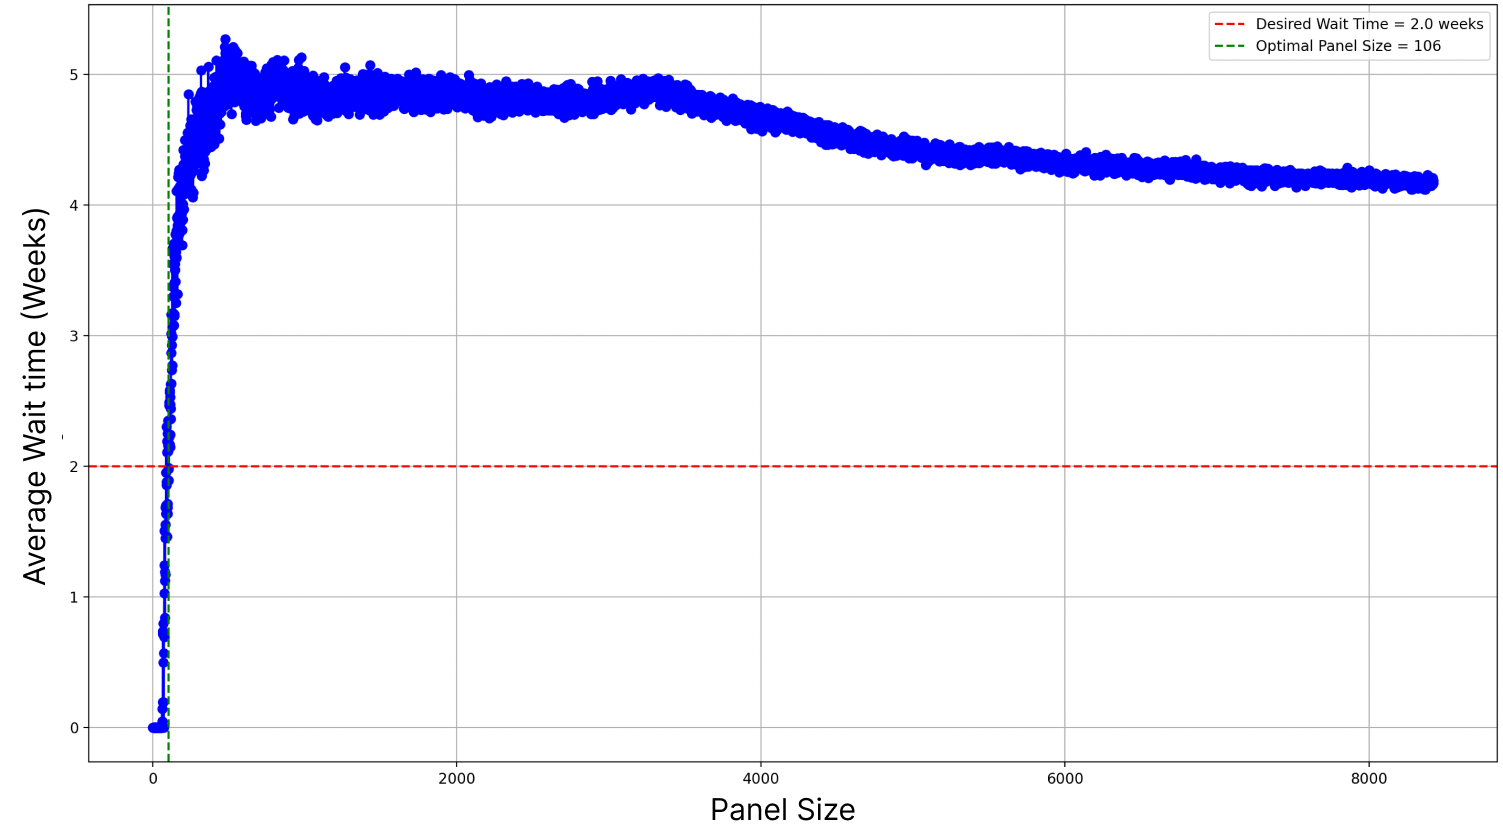
\includegraphics[width=1\textwidth]{sim1run.png}
    \caption{Panel Size vs. Average Wait time (Weeks)}
    \label{fig:show_rate}
\end{figure}

The visualization provided by the plot articulates a significant direct relationship between panel size and average wait time for appointments at VCH. As panel sizes incrementally increase, the average wait time sharply increases until a critical saturation point is reached. After this point the average wait-times start to decrease and then plateaus, suggesting a saturation point where increasing the panel size further does not significantly impact wait times. This is due to the incorporation of \text{"ShowRate"} into the simulation which sharpens the fidelity of the results, considering actual patient attendance rates, which is a critical factor in the real-world scenario.
The point highlighted by the green dashed line, marks the optimal panel size of 106, aligning with the targeted 2-week wait time signified by the red dashed line. 

\begin{figure}[H]
    \centering
    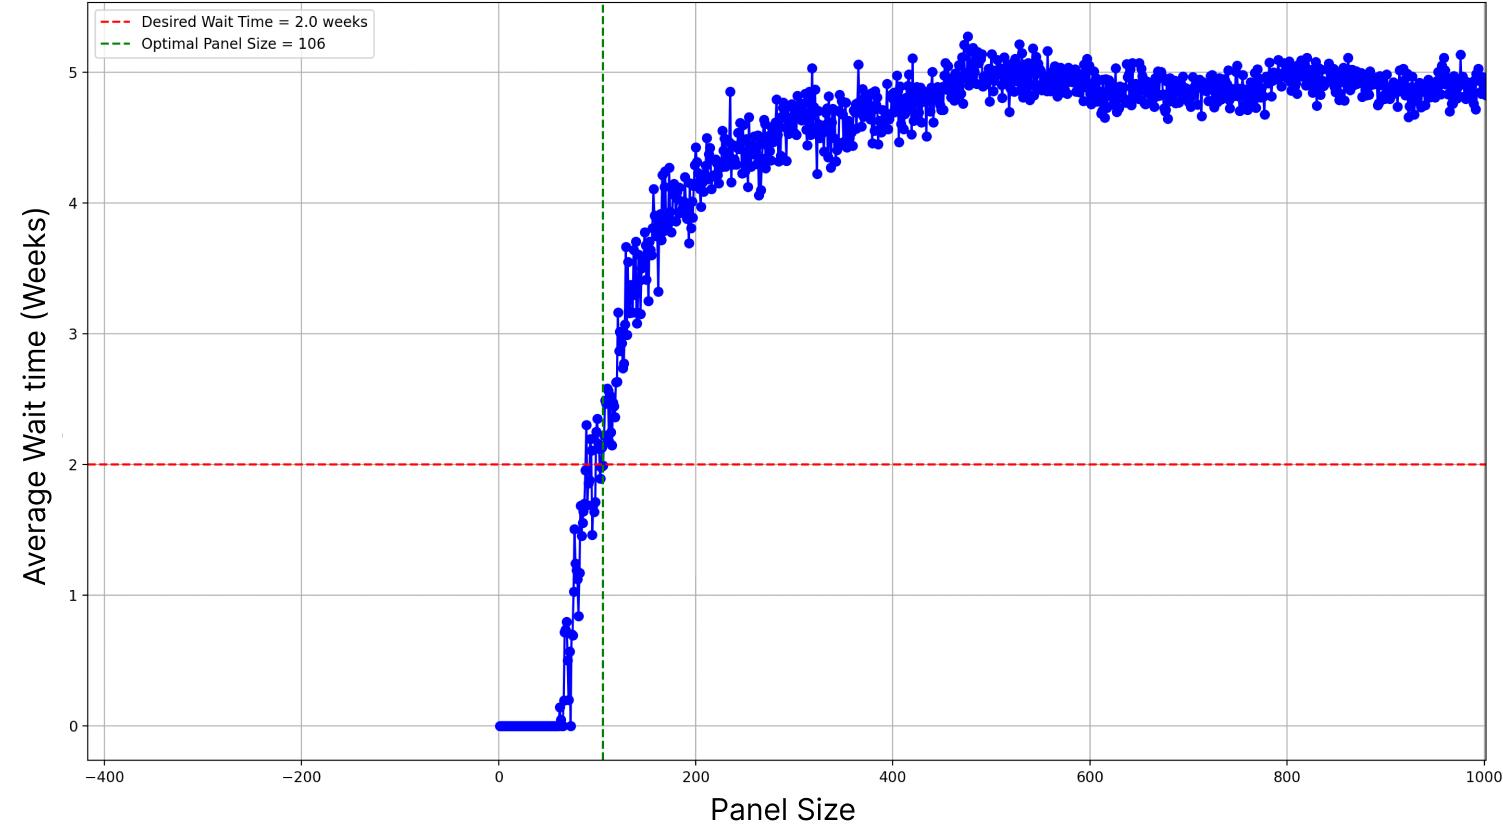
\includegraphics[width=1\textwidth]{sim1run(zoomed).png}
    \caption{Panel Size vs. Average Wait time (Weeks)}
    \label{fig:show_rate}
\end{figure}

A zoomed-in version of this plot provides a more detailed examination of this relationship, particularly within smaller panel sizes. The enhanced view reveals that the average wait time decreases more drastically as the panel sizes approach the optimal value from the larger current average of around 200. This sensitivity to panel size modifications underscores the potential benefits of operating with smaller panels.\\\\
\newpage\textbf{Stability and Variability of the Optimal Panel Size}

\begin{figure}[H]
    \centering
    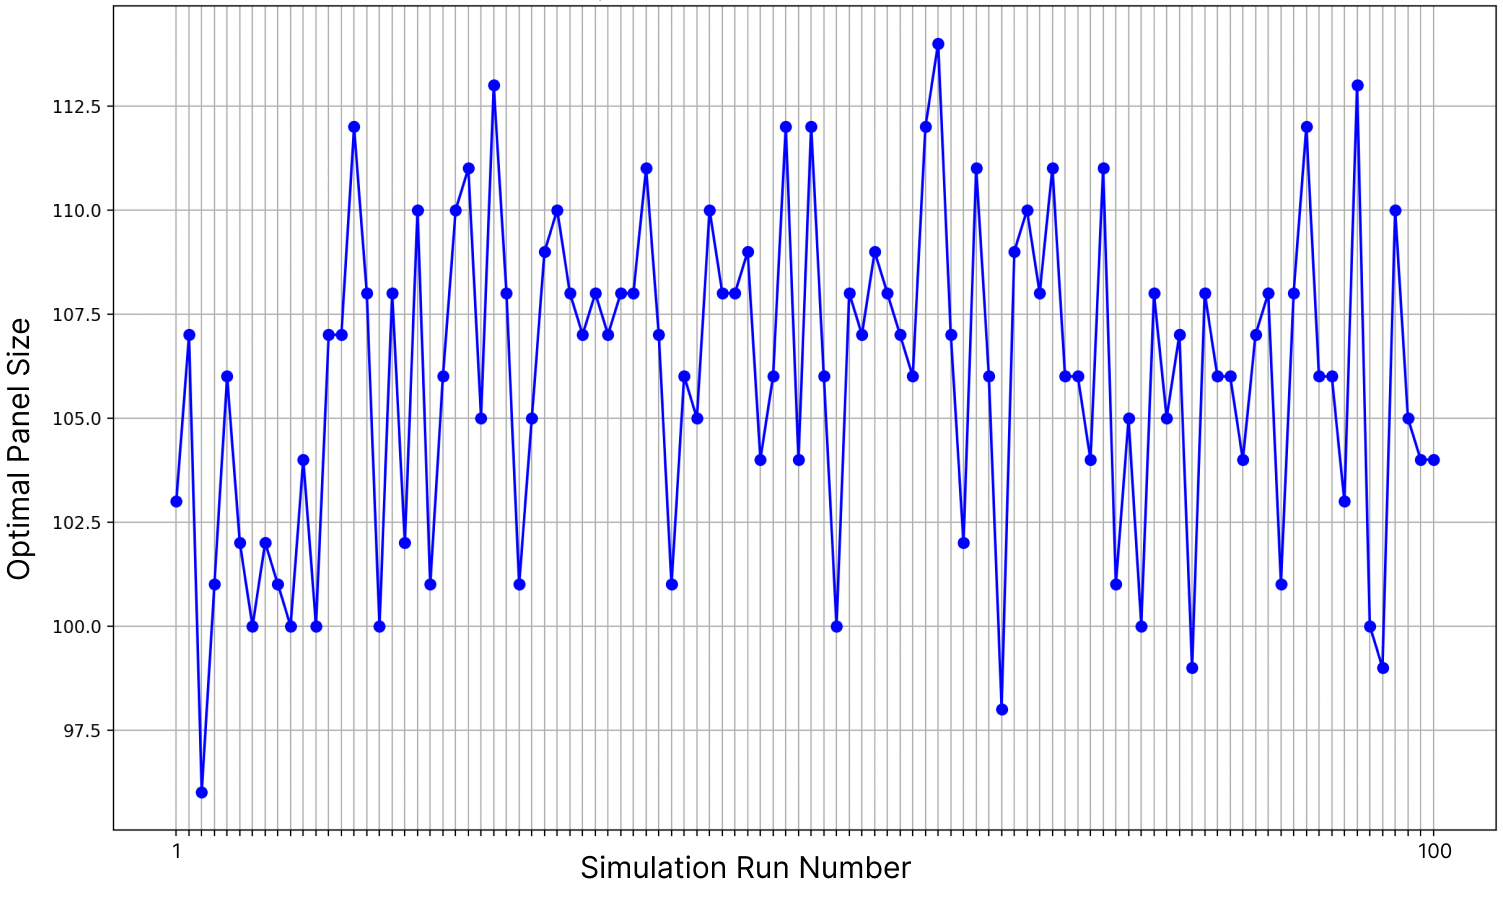
\includegraphics[width=1\textwidth]{sim100runs.png}
    \caption{Optimal panel size for 100 simulation runs.}
    \label{fig:show_rate}
\end{figure}
The third plot offers a broader perspective by simulating 100 different runs. This allows for an analysis of variance and model stability. The results of these runs exhibit a normal distribution of optimal panel sizes, predominantly clustering around 106. This confirms the robustness of the simulation model and its alignment with real-world operational dynamics, as it consistently recommends an optimal panel size within a narrow, reliable range.\\\\
\textbf{Impact of Simulation Findings}\\\\
The  simulation findings present a compelling narrative for operational enhancement at Vancouver Coastal Health (VCH), particularly concerning the optimization of Most Responsible Practitioner (MRP) panel sizes. The current state, with panels averaging around 200 patients, stands in stark contrast to the simulated ideal of 106. This significant discrepancy not only indicates the potential for a transformative change in panel structure but also highlights an opportunity for VCH to pivot toward a more patient-centric model of care.\\\\
By reducing panel sizes to align more closely with the optimal size identified through rigorous data analysis, MRPs could devote additional time to each patient, thus potentially elevating the quality of care delivered. Such personalized attention could lead to a deeper understanding of individual medical histories and needs, ultimately fostering an environment where patients are less likely to miss appointments, thereby improving the ShowRate—a key performance indicator in the healthcare domain.\\\\
The implications of moving towards smaller panel sizes are multifaceted. On one hand, it resonates with the goal of reducing no-show incidences, and on the other hand, it aligns with the patient's and healthcare provider's aspirations for a realistic and manageable two-week wait time for appointments. This target wait time, grounded in the insights gained from MRP consultations, underscores a commitment to meeting and upholding high-quality standards in patient care while simultaneously addressing patient expectations.\\\\
The impact of adhering to the optimal panel size is profound. A transition from the status quo to a more optimized panel size could result in substantial improvements in patient satisfaction, a metric that is increasingly becoming the centerpiece of healthcare evaluation. Moreover, this adjustment has the potential to balance the workload of MRPs, mitigating the risk of professional burnout and enhancing job satisfaction—both critical components in retaining a highly qualified and committed workforce.\\\\
Beyond individual practitioner benefits, the simulation findings provide a strategic roadmap for VCH to enhance the overall efficiency of healthcare delivery. By recalibrating panel sizes to the suggested optimal range, the institution could ensure that MRPs operate within a sustainable capacity, thereby utilizing hospital resources more effectively. This strategy aligns with broader objectives of hospital optimization, focusing on the dual mandate of reducing patient wait times and streamlining practitioner workloads.\\\\
In the broader context of healthcare delivery at VCH, advocating for smaller panels represents an adherence to modern healthcare optimization strategies. These strategies prioritize not just the quantitative aspects of healthcare delivery but also the qualitative nuances that influence patient satisfaction and the overall success of healthcare institutions. By fostering intimate and continuous relationships between MRPs and patients, smaller panels can cultivate a sense of trust and commitment to care, which is instrumental in achieving higher ShowRates and, by extension, a reputation for excellence in healthcare provision.\\\\
Building on these insights, Vancouver Coastal Health (VCH) is on the brink of initiating a major change in how healthcare is delivered—a change that equally values the experiences of patients and the well-being of healthcare providers. Moving toward this goal will require careful planning, involvement from important participants, and a step-by-step approach to track progress and effects. The main aim is clear: to create a healthcare system that is both effective and caring, placing VCH as a leader in focusing on the needs of patients.


\section{Limitations and Further Direction}
While this study provides significant insights into optimizing MRP panel sizes and understanding the impact of patient complexity and appointment adherence on healthcare delivery, it is not without limitations. Acknowledging these limitations is crucial for contextualizing the findings and guiding future research efforts.\\\\

\textbf{Limitations:}

\begin{itemize}

\item Data Scope and Representation: The analysis was based on Electronic Medical Records EMR data provided by VCH, focusing on a defined set of appointment types (scheduled appointments) and excluding non-clinical interactions and walk-ins. While this approach enhances the specificity of the lambda and ShowRate calculations, it may also limit the generalizability of our findings across different healthcare settings or patient populations. Furthermore, the complexity of healthcare needs, CSI and appointment adherence ShowRate are dynamic metrics that can evolve over time, influenced by factors beyond the scope of this dataset.

\item Fixed Time for Appointments: Our simulations assumed a standardized thirty-minute slot for all appointments based on practitioner feedback. This assumption does not account for the variability in appointment durations that may be necessary for addressing complex healthcare needs. The fixed appointment time model might oversimplify the intricacies of real-world healthcare delivery, where some conditions require longer consultations.

\item Exclusion of certain appointment types in ShowRate Calculation: While refining the ShowRate by excluding certain appointment types aimed to provide a more accurate measure of patient engagement, this approach may inadvertently overlook the underlying reasons for no-shows. Understanding the causes of missed appointments is critical for developing more effective strategies to enhance patient attendance and engagement. Patients could miss a scheduled appointment and show up for walk-in on the same day itself. A detailed analysis of each patient and their appointment booking habits could give us more detailed insights. A simulation that considers patient's behavioural trend in context of appointment booking and attending the appointments, could provide us with a more accurate simulation.

\item Limited Integration of CSI Complexity in Simulation: Although we successfully calculated the Complexity Score Index (CSI) for patients, integrating this complexity into our simulation model proved challenging due to its dependence on multi-factorial aspects. The CSI encompasses variables such as the PR Index, indicating the breadth of programs and referrals a patient is associated with; the "V Index", reflecting the volume of services accessed by a patient; the "EA index, denoting emergency needs; the "DCR index", capturing the diagnosis service risk; and the "Formal risk", assessing the threshold of mental health risks like overdose events. These factors collectively contribute to a patient's healthcare complexity but were not directly incorporated into our simulation. The omission is primarily due to the intricate nature of these variables and their dynamic interplay, which complicates their direct application in determining panel sizes and scheduling efficiencies. This limitation underscores the need for advanced simulation models that can adeptly navigate the complexities of healthcare needs and integrate multifaceted patient risk assessments to optimize MRP panel sizes and healthcare delivery strategies.
\end{itemize}
\textbf{Future Directions:}
\begin{itemize}
\item Expanding the Data Source: Future research could benefit from incorporating a broader dataset that includes a wider variety of healthcare settings, appointment types, and patient demographics. This expansion would enhance the robustness of the lambda and CSI calculations and provide a more comprehensive understanding of patient needs and behaviors.

\item Investigating the Reasons for No-Shows: A qualitative study exploring the reasons behind patient no-shows could offer valuable insights into improving appointment adherence \cite{Liu2014}. Understanding patient barriers to attending scheduled appointments could inform targeted interventions to reduce no-show rates and optimize healthcare delivery.

\item Dynamic Appointment Scheduling Models: Exploring models that allow for variable appointment duration based on the complexity of the patient's needs could lead to more efficient and effective healthcare provision \cite{Abdalkareem2021, Luo2017}. Research into dynamic scheduling systems that adapt to the real-time demand and complexity of care could significantly improve patient outcomes and practitioner well-being.

\item Integration of Patient Feedback: Incorporating patient feedback on their healthcare experiences, especially regarding appointment scheduling and wait times, could offer critical insights into optimizing panel sizes. Patient-centered research could reveal preferences and expectations that inform more responsive healthcare delivery models. \cite{Angstman2016}

\item Advanced Simulation Models Incorporating CSI: Developing more sophisticated simulation models that can incorporate the Complexity Score Index (CSI) along with its underlying factors—such as PR Index, V Index, "EA index", "DCR index", and "Formal risk" is essential. Future models should aim to dynamically account for the multifaceted aspects of patient complexity and risk factors, potentially through machine learning algorithms or complex system simulations. This advancement would allow for more accurate predictions of healthcare needs and more efficient resource allocation \cite{humphreys2022}.

\item Integration of Real-time Data and Predictive Analytics: Leveraging real-time EMR data and predictive analytics could enable a dynamic adjustment of panel sizes and scheduling in response to evolving healthcare demands and patient complexity. This direction would involve the continuous update and refinement of models based on current data trends.

\item Patient-Centered Care Models: Investigating models that prioritize patient-centered care by integrating patient preferences, satisfaction scores, and outcome measures into the analysis. This approach would aim to balance operational efficiency with patient satisfaction and healthcare outcomes, ensuring that the system evolves in alignment with patient needs.

\item Cross-Setting Generalizability Studies: Conduct studies to assess the generalizability of the findings across different healthcare settings, geographical areas, and healthcare systems. This could help validate the models developed and ensure their applicability in diverse contexts.

\item Collaborative Healthcare Frameworks: Explore the development of collaborative frameworks that involve multidisciplinary teams in the care process, considering the broader spectrum of patient needs as indicated by CSI. This could include integrated care pathways that involve specialists, mental health professionals, and social services to address the comprehensive needs of patients.

By addressing these limitations and pursuing the outlined future directions, subsequent research has the potential to significantly advance our understanding of optimal healthcare delivery. Building on the foundations laid by this study, future efforts can continue to explore innovative strategies for balancing healthcare demand with practitioner capacity, ultimately contributing to a more efficient, effective, and patient-centered healthcare system.
\end{itemize}



\section{Discussion}
The task of optimizing panel sizes for Most Responsible Practitioners (MRPs) within the Vancouver Coastal Health (VCH) network is a complex challenge with significant implications for the efficiency of healthcare delivery and patient outcomes. This study embarked on an in-depth exploration, utilizing advanced methodologies such as discrete event simulation (DES) and the Poisson distribution, to delve into the intricate dynamics of panel size management. Through comprehensive data analysis and simulation, we aimed to address pressing concerns regarding workload management for MRPs and patient care quality within the VCH network. \\

Our findings underscore the critical importance of optimizing panel sizes to strike a delicate balance between patient demand and practitioner capacity. The nonlinear relationship between panel size and average wait times for appointments highlights the need for nuanced panel size determination strategies. While larger panel sizes may initially accommodate higher patient loads, our simulations reveal diminishing returns beyond a certain threshold, ultimately leading to longer wait times and potential strains on practitioner well-being. Conversely, smaller panel sizes may offer more personalized care and shorter wait times but may pose challenges in efficiently managing patient demand, particularly in high-volume settings. \\

Furthermore, our study elucidates the complexitiesappointment’s  in healthcare delivery dynamics and the challenges associated with accurately modeling real-world scenarios. Limitations such as data scope constraints, fixed appointment durations, and the exclusion of certain appointment types in show rate calculations underscore the need for continuous refinement and validation of simulation models. Despite these limitations, our study provides valuable insights into the factors influencing panel size determination and offers a foundation for future research endeavors aimed at addressing these challenges.


\section{Conclusion}
In light of the findings from this study, several future research directions emerge that hold the potential to further enhance our understanding of optimal panel size determination and healthcare delivery efficiency. Expanding the scope of data sources to encompass a broader spectrum of healthcare settings and patient demographics could provide a more comprehensive understanding of patient needs and behaviors. Integration of real-time data and predictive analytics offers promise for dynamically adjusting panel sizes in response to evolving healthcare demands, thereby improving the responsiveness and efficiency of healthcare delivery systems. \\

Moreover, exploring patient-centered care models and collaborative healthcare frameworks involving multidisciplinary teams represents an innovative approach to optimize healthcare delivery further. By prioritizing patient preferences, satisfaction scores, and outcome measures, these models aim to balance operational efficiency with patient-centered care, ultimately fostering a more holistic and patient-centric approach to healthcare delivery. \\

In conclusion, this study represents a crucial step towards optimizing panel sizes for MRPs within the VCH network. By leveraging advanced simulation methodologies and data-driven insights, we have provided valuable recommendations for enhancing healthcare delivery efficiency and patient outcomes. Continued efforts in this direction, coupled with ongoing refinement of simulation models and exploration of innovative healthcare delivery strategies, hold the potential to transform healthcare delivery paradigms and foster a more efficient, effective, and patient-centered healthcare system within the VCH network and beyond. \\

\newpage

\bibliographystyle{plainnat}
\bibliography{references}

\newpage
% Start of the appendix
\section{Appendix}

\subsection*{Project Repository}
For more information, see the project on GitHub:\url{https://github.com/npsadafule/Math402W.git}

\subsection*{Pseudocode}
\begin{algorithm}
\caption{Pseudo code to calculate the Rate of booking appointments ($\lambda$) and Complexity score Index (CSI) }
\begin{algorithmic}[1]

\State Load lambda data from 'Appointments.xlsx' using specific columns
\State Convert 'ApptBookedDate' to datetime objects
\State Define a list of appointment types to be excluded
\State Filter the data to exclude certain appointment types

\State Define start and end dates for the period covered
\State Calculate the total number of months in the period
\State Group lambda data by 'PID' and count occurrences
\State Calculate lambda for each patient by dividing occurrences by total months
\State Reset index on lambda data to create a clean dataframe

\State Load CSI data from 'CSI data.xlsx' using specific columns
\State Group CSI data by 'PID' and calculate the mean score
\State Reset index on CSI data to create a clean dataframe

\State Connect to MongoDB and select healthcare database and patients collection

\For{each patient in lambda data}
    \State Update lambda values in the MongoDB patients collection
\EndFor

\For{each patient in CSI data}
    \State Update CSI scores in the MongoDB patients collection
\EndFor

\State Close MongoDB connection
\State Print message indicating database update completion

\end{algorithmic}
\end{algorithm}
\newpage
\begin{algorithm}
\caption{Calculate Patient Show Rates}
\begin{algorithmic}[1]

\State Load appointment data from 'Appointments.xlsx' into a dataframe with columns 'PID', 'is visit', and 'ApptTypeDesc'
\State Define a list of appointment types that are to be excluded from calculations
\State Filter out appointments from the dataframe that are in the excluded types list
\State Group the filtered dataframe by 'PID'
\State Calculate the show rate as the average of 'is visit' values for each 'PID'
\State Rename the mean 'is visit' column to 'ShowRate' in the show rate dataframe
\State Establish a connection to the MongoDB database and specify the 'patients' collection
\For{each patient in the show rate dataframe}
    \State Update the MongoDB for the patient with the 'ShowRate'
\EndFor
\State Print a message indicating that the database update is complete
\State Close the MongoDB connection

\end{algorithmic}
\end{algorithm}
\newpage
\begin{algorithm}
\caption{Pseudo-code for the Simulation}
\begin{algorithmic}[1]

\State \textbf{Inputs:} Desired wait time
\State \textbf{Output:} Optimal panel size to achieve desired wait time

\Procedure{}{}
    \State Prompt user for desired\_wait\_time
    \State Connect to MongoDB and select healthcare database and patients collection
    \State Fetch Lambda and ShowRate values for all patients
    \State Close MongoDB connection
    \State Set hours\_per\_week based on MRP availability
    \State Set slots\_per\_week assuming 30 mins per appointment
    \State Set weeks for simulation period (16 weeks)
    \State Calculate total\_slots as slots\_per\_week $\times$ weeks
    \State Define function simulate\_panel\_size to estimate wait times:
    \State \hspace{\algorithmicindent} Takes panel\_size, lambdas, show\_rates, and total\_slots as inputs
    \State \hspace{\algorithmicindent} Calculates the total requested appointments
    \State \hspace{\algorithmicindent} Returns the calculated wait time
    \State Initialize empty lists for panel\_sizes and average\_wait\_times
    \State Initialize optimal\_panel\_size as None
    \For{each possible panel size from largest to smallest}
        \State Calculate wait time using simulate\_panel\_size
        \State Record the panel size and the calculated wait time
        \If{current panel size achieves the desired wait time}
            \State Set optimal\_panel\_size to current panel size
        \EndIf
    \EndFor

    \State Plot panel sizes against average wait times
    \State Highlight the desired wait time and optimal panel size if one exists
    \If{an optimal panel size was found}
        \State Print the optimal panel size
    \Else
        \State Print that no panel size can achieve the desired wait time
    \EndIf
\EndProcedure
\end{algorithmic}
\end{algorithm}


\end{document}
